\PassOptionsToPackage{table}{xcolor}

\documentclass[
%	handout,
	notes=none,
	aspectratio=169
]{beamer}

% Comment out the following line to hide the notes
%\setbeameroption{show notes}

\input{macros}

\usefolder{theme}
\usetheme{sailfish}

\begin{document}

\title{Daily blogging embedded Gecko development}
\subtitle{FOSDEM'24\\FOSS on Mobile Devroom}
\author{David Llewellyn-Jones}
\date{3rd February 2024}

%%%%%%%%%%%%%%%%%%%%%%%%%%%%%%%%%%%%%%%%%

\renewcommand{\thefootnote}{\arabic{footnote}}

\frame{
\titlepage
}
\note{
}

\renewcommand{\thefootnote}{\fnsymbol{footnote}}

%%%%%%%%%%%%%%%%%%%%%%%%%%%%%%%%%%%%%%%%%

\begin{frame}
\frametitle{About me}

\begin{columns}[T]
\begin{column}[T]{0.4\textwidth}
\setlength{\parskip}{0.5em}

\vspace{1.0cm}
\begin{enumerate}
\setlength{\parskip}{0.5em}
\item Software Engineer for Jolla until a year ago
\item Now a Research Data Scientist for The Alan Turing Instutaute
\end{enumerate}
\ \ \ \url{https://www.flypig.co.uk}

\end{column}
\begin{column}[T]{0.6\textwidth}
\setlength{\parskip}{0.5em}

\vspace{0.5cm}
\begin{center}

\includegraphics[width=1.0\textwidth]{aboutme}
\end{center}

\end{column}
\end{columns}

\end{frame}
\note{
\begin{enumerate}
\item My last day at Jolla was spent at FOSDEM'23.
\item Jolla develops Sailfish OS.
\end{enumerate}
}

%%%%%%%%%%%%%%%%%%%%%%%%%%%%%%%%%%%%%%%%%

\begin{frame}
\frametitle{Sailfish OS}

\begin{columns}[T]
\begin{column}[T]{0.5\textwidth}
\setlength{\parskip}{0.5em}

\vspace{1.5cm}
\begin{enumerate}
\setlength{\parskip}{0.5em}
\item Linux smartphone OS
\item {\tt glibc}, {\tt busybox}
\item A descendant of Maemo
\item Default {\tt sailfish-browser} is gecko-based
\end{enumerate}

%\vspace{0.5cm}
%\includegraphics[width=1.0\textwidth]{pillars}

\end{column}
\begin{column}[T]{0.5\textwidth}
\setlength{\parskip}{0.5em}

\vspace{0.5cm}
\includegraphics[width=1.0\textwidth]{stack}

\end{column}
\end{columns}

\end{frame}
\note{
\begin{enumerate}
\item A Linux smartphone operating system released in 2012.
\item {\tt glibc}, {\tt busbox}, native or libhybris.
\item When I was at Jolla I wortked on many different things, including: user interface, core apps, email client, Exchange support, Settings app, cloud sync.
\item I also worked on the Web browser, called {\tt sailfish-browser}, based on the gecko rendering engine.
\end{enumerate}
}

%%%%%%%%%%%%%%%%%%%%%%%%%%%%%%%%%%%%%%%%%

\begin{frame}
\frametitle{Gecko}

\begin{columns}[T]
\begin{column}[T]{0.5\textwidth}
\setlength{\parskip}{0.5em}

\vspace{1.5cm}
\begin{enumerate}
\setlength{\parskip}{0.5em}
\item Mozilla's rendering engine used in Firefox
\item Released in 2000, Netscape 6
\item Alternative to Blink, WebKit, Netsurf
\end{enumerate}

\end{column}
\begin{column}[T]{0.5\textwidth}
\setlength{\parskip}{0.5em}

\vspace{0.5cm}
\includegraphics[width=1.0\textwidth]{mozilla}

\end{column}
\end{columns}

\end{frame}
\note{
\begin{enumerate}
\item Mozilla's rendering engine used in Firefox
\item First appeared in 2000 with the release of Netscape 6
\item Alternative to Blink (Chrome, Edge, Brave, Vivaldi), WebKit (Safari, iOS, Ephiphany), Netsurf (Netsurf)
\end{enumerate}
}

%%%%%%%%%%%%%%%%%%%%%%%%%%%%%%%%%%%%%%%%%

\begin{frame}
\frametitle{Gecko on Sailfish OS}

\begin{columns}[T]
\begin{column}[T]{0.6\textwidth}
\setlength{\parskip}{0.5em}

\vspace{1.5cm}
\begin{enumerate}
\setlength{\parskip}{0.5em}
\item Artefact of Sailfish OS's Maemo history
\item Based on EmbedLite and XULRunner
\end{enumerate}

\end{column}
\begin{column}[T]{0.4\textwidth}
\setlength{\parskip}{0.5em}

\vspace{0.0cm}
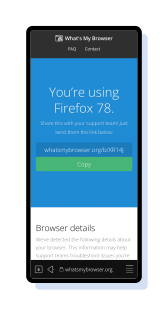
\includegraphics[height=0.9\textheight]{esr78}

\end{column}
\end{columns}

\end{frame}
\note{
\begin{enumerate}
\item Artefact of Sailfish OS's Maemo history.
\item microB browser on the n900.
\item Based on EmbedLite and XULRunner.
\item XULRunner the library version of the renderer; EmbedLite the embedding mechanism.
\item Embedding mechanism allows gecko to be embedded in other applications running on a separate thread or separate process.
\end{enumerate}
}

%%%%%%%%%%%%%%%%%%%%%%%%%%%%%%%%%%%%%%%%%

\begin{frame}
\frametitle{Embedding Gecko}

\begin{columns}[T]
\begin{column}[T]{1.0\textwidth}
\setlength{\parskip}{0.5em}

\vspace{0.5cm}

\begin{shadequote}[r]{Chris Lord, February 2016}
Gecko has limited embedding capability that is not well-documented, not well-maintained and not heavily invested in... We have at various points in history had embedding APIs/capabilities, but we have either dropped them (gtkmozembed) or let them bit-rot (IPCLite).
\end{shadequote}

\end{column}
\end{columns}

\end{frame}
\note{
\begin{enumerate}
\item It's an old quote, but holds true today.
\item Chris Lord was a Mozilla engineer at the time.
\item He makes clear he's not criticising the implementations, but rather the strategic direction of Mozilla.
\item IPCLite is another name for EmbedLite.
\item \url{https://www.chrislord.net/2016/02/24/the-case-for-an-embeddable-gecko/}
\item \url{https://www.chrislord.net/2016/03/08/state-of-embedding-in-gecko/}
\end{enumerate}
}

%%%%%%%%%%%%%%%%%%%%%%%%%%%%%%%%%%%%%%%%%

\begin{frame}
\frametitle{Sailfish Browser}

\begin{columns}[T]
\begin{column}[T]{1.1\textwidth}

\vspace{0.5cm}
\includegraphics[width=1.0\textwidth]{components}

\end{column}
\end{columns}

\end{frame}
\note{
\begin{enumerate}
\item The Sailfish Browser isn't just gecko.
\item {\tt sailfish-browser} provides the user interface (C++/Qt/QML).
\item {\tt embedlite-components} provides JavaScript user interface functionality (JavaScript).
\item {\tt qtmozembed} turns gecko into an embeddable Qt component (C++/Qt).
\item {\tt gecko} is the EmbedLite embedded gecko renderer (JavaScript/C++/Rust).
\end{enumerate}
}

%%%%%%%%%%%%%%%%%%%%%%%%%%%%%%%%%%%%%%%%%

\begin{frame}
\frametitle{Sailfish Browser}

\begin{columns}[T]
\begin{column}[T]{1.1\textwidth}

\vspace{0.5cm}
\includegraphics[width=1.0\textwidth]{languages}

\end{column}
\end{columns}

\end{frame}
\note{
\begin{enumerate}
\item The Sailfish Browser isn't just gecko.
\item {\tt sailfish-browser} provides the user interface (C++/Qt/QML).
\item {\tt embedlite-components} provides JavaScript user interface functionality (JavaScript).
\item {\tt qtmozembed} turns gecko into an embeddable Qt component (C++/Qt).
\item {\tt gecko} is the EmbedLite embedded gecko renderer (JavaScript/C++/Rust).
\end{enumerate}
}

%%%%%%%%%%%%%%%%%%%%%%%%%%%%%%%%%%%%%%%%%

\begin{frame}
\frametitle{The Upgrade Problem}

\begin{columns}[T]
\begin{column}[T]{1.0\textwidth}
\setlength{\parskip}{0.5em}

\vspace{1.5cm}
\begin{enumerate}
\setlength{\parskip}{0.5em}
\item Sailfish Browser ESR 60: February 2021
\item Sailfish Browser ESR 78: March 2022
\item Latest Firefox ESR: 115
\item By my estimate upgrading takes ~36 person-months
\end{enumerate}

\end{column}
\end{columns}

\end{frame}
\note{
\begin{enumerate}
\item ESR stands for Extended Support Release, a gecko naming convention.
\item ESRs released roughly every 10 release cycles.
\item Supported for 12 weeks after next ESR release.
\item Receive security updates but not new features.
\item The Sailfish Browser has received semi-regular updates.
\item It was upgraded to ESR 60 in February 2021 and ESR 78 in March 2022.
\item However the most recent gecko ESR is 115.
\item Upgrading is a {\it lot\/} of work, mostly because of the patching required.
\item As gecko diverged from EmbedLite, patching increased; now have 99 patches, 104845 lines of diff.
\item Upgrading takes (my guess) around 36 person-months.
\end{enumerate}
}

%%%%%%%%%%%%%%%%%%%%%%%%%%%%%%%%%%%%%%%%%

\begin{frame}
\frametitle{Starting Out}

\begin{columns}[T]
\begin{column}[T]{1.0\textwidth}
\setlength{\parskip}{0.5em}

\vspace{1.5cm}
\begin{enumerate}
\setlength{\parskip}{0.5em}
\item In August I decided to attempt the upgrade from ESR 78 to ESR 91
\item Hoping my experience with 60 and 78 might help
\item I didn't want to do it alone
\end{enumerate}

\end{column}
\end{columns}

\end{frame}
\note{
\begin{enumerate}
\item In August I decided to attempt the upgrade from ESR 78 to ESR 91.
\item Hoping my experience with 60 and 78 might help.
\item I didn't want to do it alone; so I decided to write a daily dev diary.
\end{enumerate}
}

%%%%%%%%%%%%%%%%%%%%%%%%%%%%%%%%%%%%%%%%%

\begin{frame}
\frametitle{What is a Dev Diary?}

\begin{columns}[T]
\begin{column}[T]{1.0\textwidth}
\setlength{\parskip}{0.5em}

\vspace{1.5cm}
\begin{shadequote}[r]{Jay Wilson, January 2023}
A developer diary is where you write about developer things. It can be the record of what you worked on last, some decisions made by steak-holders in the product, and or a neat way to accomplish a task. It really comes down to what you want to put in it.
\end{shadequote}

\end{column}
\end{columns}

\end{frame}
\note{
\begin{enumerate}
\item Dev diaries are common in the gaming community.
\item My first experience of a dev diary was with the crowd-funded Prison Architect in 2012.
\item Producer Mark Morris and Designer Chris Delay vlogged progress.
\item In the game industry they're often a marketing tool.
\item But my motiviation was different: first to help me code; second to involve the Sailfish community.
\end{enumerate}
}

%%%%%%%%%%%%%%%%%%%%%%%%%%%%%%%%%%%%%%%%%

\begin{frame}
\frametitle{Helping Me Code}

\begin{columns}[T]
\begin{column}[T]{1.0\textwidth}
\setlength{\parskip}{0.5em}

\vspace{1.5cm}
\begin{enumerate}
\setlength{\parskip}{0.5em}
\item Aide-mémoire
\item Build a searchable record of changes
\item Encourage structured thoughts
\item Motivate daily work
\end{enumerate}

\end{column}
\end{columns}

\end{frame}
\note{
\begin{enumerate}
\item Help me remember what I'm doing day-to-day.
\item Force me to write down my processes every day.
\item Make me think about what I'm doing and help structure my thoughts.
\item Work consistently.
\end{enumerate}
}

%%%%%%%%%%%%%%%%%%%%%%%%%%%%%%%%%%%%%%%%%

\begin{frame}
\frametitle{Involve the Community}

\begin{columns}[T]
\begin{column}[T]{1.0\textwidth}
\setlength{\parskip}{0.5em}

\vspace{1.5cm}
\begin{enumerate}
\setlength{\parskip}{0.5em}
\item Browser upgrades are important
\item Users want to know about progress
\item Allow others to help
\end{enumerate}

\end{column}
\end{columns}

\end{frame}
\note{
\begin{enumerate}
\item Browser upgrades are seen as important by the community.
\item Having to wait, without any idea of progress, for the next browser is frustrating.
\item I needed help with: coding ideas; testing; other components (e.g. gcc, Rust); motiviation.
\end{enumerate}
}

%%%%%%%%%%%%%%%%%%%%%%%%%%%%%%%%%%%%%%%%%

\begin{frame}
\frametitle{Downsides}

\begin{columns}[T]
\begin{column}[T]{1.0\textwidth}
\setlength{\parskip}{0.5em}

\vspace{1.5cm}
\begin{enumerate}
\setlength{\parskip}{0.5em}
\item Coding this way takes about twice as long
\item Daily updates are great motivation, but also a bind
\item Best for tasks that can be split into daily pieces
\item Visual output helps
\end{enumerate}

\end{column}
\end{columns}

\end{frame}
\note{
\begin{enumerate}
\item Having to write everything down is time-consuming and makes coding take longer.
\item It's great to force yourself to work on something, but on some days it can be gruelling.
\item Challenging tasks that require a lot of thought to fix don't work so well.
\item Having visual results to share is great; which may explain why they're so popular in the games industry.
\end{enumerate}
}

%%%%%%%%%%%%%%%%%%%%%%%%%%%%%%%%%%%%%%%%%

\begin{frame}
\frametitle{Timeline}

\begin{columns}[T]
\begin{column}[T]{1.0\textwidth}

\vspace{0.2cm}

\includegraphics[width=1.0\textwidth]{timeline}

\end{column}
\end{columns}

\end{frame}
\note{
\begin{enumerate}
\item TBC.
\end{enumerate}
}

%%%%%%%%%%%%%%%%%%%%%%%%%%%%%%%%%%%%%%%%%

\begin{frame}
\frametitle{Community Response}

\begin{columns}[T]
\begin{column}[T]{1.0\textwidth}
\setlength{\parskip}{0.5em}

\vspace{1.5cm}
\begin{enumerate}
\setlength{\parskip}{0.5em}
\item Utterly overwhelming
\item People are so generous and nice
\item Did I join the wrong Internet?
\end{enumerate}

\end{column}
\end{columns}

\end{frame}
\note{
\begin{enumerate}
\item The response has been absolutely amazing.
\item I actually am surprised anyone reads the diary entries; they're technical and I don't tone them down at all.
\item Users have helped solve problems; share ideas; test builds; generated blog content and graphics.
\item Sometimes I think I inhabit a different Internet to the one portrayed in the media.
\end{enumerate}
}

%%%%%%%%%%%%%%%%%%%%%%%%%%%%%%%%%%%%%%%%%

\begin{frame}
%\frametitle{Thigg's Images}

\begin{columns}[T]
\begin{column}[T]{1.0\textwidth}

\vspace{-0.12cm}
\hspace*{-1.1cm}
\includegraphics[width=1.15\textwidth]{Thigg}

\end{column}
\end{columns}

\end{frame}
\note{
\begin{enumerate}
\item A special shout-out to Thigg who has been created AI-generated images to go alongside my blog posts. They are amazing.
\end{enumerate}
}

%%%%%%%%%%%%%%%%%%%%%%%%%%%%%%%%%%%%%%%%%

\begin{frame}
\frametitle{Demo}

\begin{columns}[T]
\begin{column}[T]{1.0\textwidth}

\vspace{0.5cm}
\begin{center}
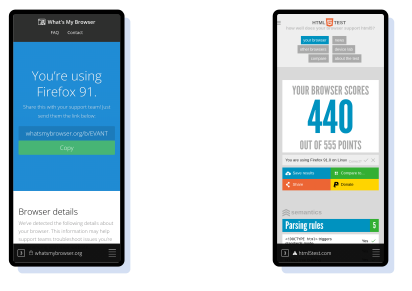
\includegraphics[width=0.65\textwidth]{esr91}
\end{center}

\end{column}
\end{columns}

\end{frame}
\note{
\begin{enumerate}
\item Live demo if possible using Screencast.
\end{enumerate}
}

%%%%%%%%%%%%%%%%%%%%%%%%%%%%%%%%%%%%%%%%%

\begin{frame}
\frametitle{Closing Thoughts}

\begin{columns}[T]
\begin{column}[T]{1.0\textwidth}
\setlength{\parskip}{0.5em}

\vspace{1.5cm}
\begin{enumerate}
\setlength{\parskip}{0.5em}
\item Writing a dev diary is great for open source
\item It's not literature, it's code
\item Work a couple of entries in advance
\item Stick to a strict cadence
\item Write about what your tommorrow-self will need to know
\end{enumerate}

\end{column}
\end{columns}

\end{frame}
\note{
\begin{enumerate}
\item A dev diary is especially good for open source projects where you can share code and others can contribute.
\item Some may be put off for fear of having to write interesting topics. That doesn't bother me because I don't. I just write what I do.
\item Work a couple of entries in advance.
\item Stick to a strict cadence.
\item Write about things that you think might help if you were to refer back to them tomorrow or in the future.
\end{enumerate}
}

%%%%%%%%%%%%%%%%%%%%%%%%%%%%%%%%%%%%%%%%%

\begin{frame}
\frametitle{Thank You!}

\begin{columns}[T]
\begin{column}[T]{1.1\textwidth}

\vspace{-0.5cm}
\includegraphics[width=1.0\textwidth]{thanks}

\end{column}
\end{columns}

\end{frame}
\note{
\begin{enumerate}
\item Thank you to everyone who's been reading my diaries, made suggestions, helped, supported and motivated me.
\end{enumerate}
}

%%%%%%%%%%%%%%%%%%%%%%%%%%%%%%%%%%%%%%%%%

\begin{frame}[fragile]
\frametitle{Further info}
\setlength{\leftmargini}{7.0em}
\vspace{0.8cm}

\begin{itemize}
\setlength{\parskip}{1.0em}
\item[Dev Diary] \, \url{https://www.flypig.co.uk/gecko}
\item[Sailfish Browser] \, \url{https://github.com/sailfishos/sailfish-browser}
\item[Gecko source] \, \url{https://github.com/llewelld/gecko-dev}
\item[Sailfish OS] \, \url{https://sailfishos.org}
\item[Slides source] \, \url{https://github.com/llewelld/fosdem24-gecko-dev}
\end{itemize}

\end{frame}
\note{
\fontsize{7pt}{8pt}{\bibliographystyle{ieeetr}}
\bibliography{slides}
}

%%%%%%%%%%%%%%%%%%%%%%%%%%%%%%%%%%%%%%%%%

\end{document}
